\documentclass[aspectratio=169]{beamer}
\usepackage{lmodern}
\usetheme{Madrid}
%\usecolortheme{giantoak}
\newcommand*\oldmacro{}
\let\oldmacro\insertshorttitle
\renewcommand*\insertshorttitle{\oldmacro\hfill\insertframenumber\,/\,\inserttotalframenumber}
\usepackage[framemethod=tikz]{mdframed}

\usepackage{beamerthemesplit}
\usepackage{textpos}
\usepackage{pgf}
%\logo{\pgfputat{\pgfxy(0,-.4)}{\pgfbox[right,base]{\includegraphics[height=1.0cm]{logo.jpg}}}}
%\newcommand{\nologo}{\setbeamertemplate{logo}{}}
\usepackage{booktabs}
\usepackage{graphicx}
\theoremstyle{principle}
\newtheorem*{principle}{Design Principle}


\titlegraphic{\includegraphics[width=1.0\paperwidth]{cool-wind-800px.jpg}}

\title{Amendments}
%\author[Jeremy Kedziora]{Wind Data Science Team\\
%\small{Uptake}}
\date{}

\begin{document}

%{
%%\nologo
%\begin{frame}
%    \maketitle
%\end{frame}
%}
%pages 1-7, 8-9, 14-15.


{
  \usebackgroundtemplate{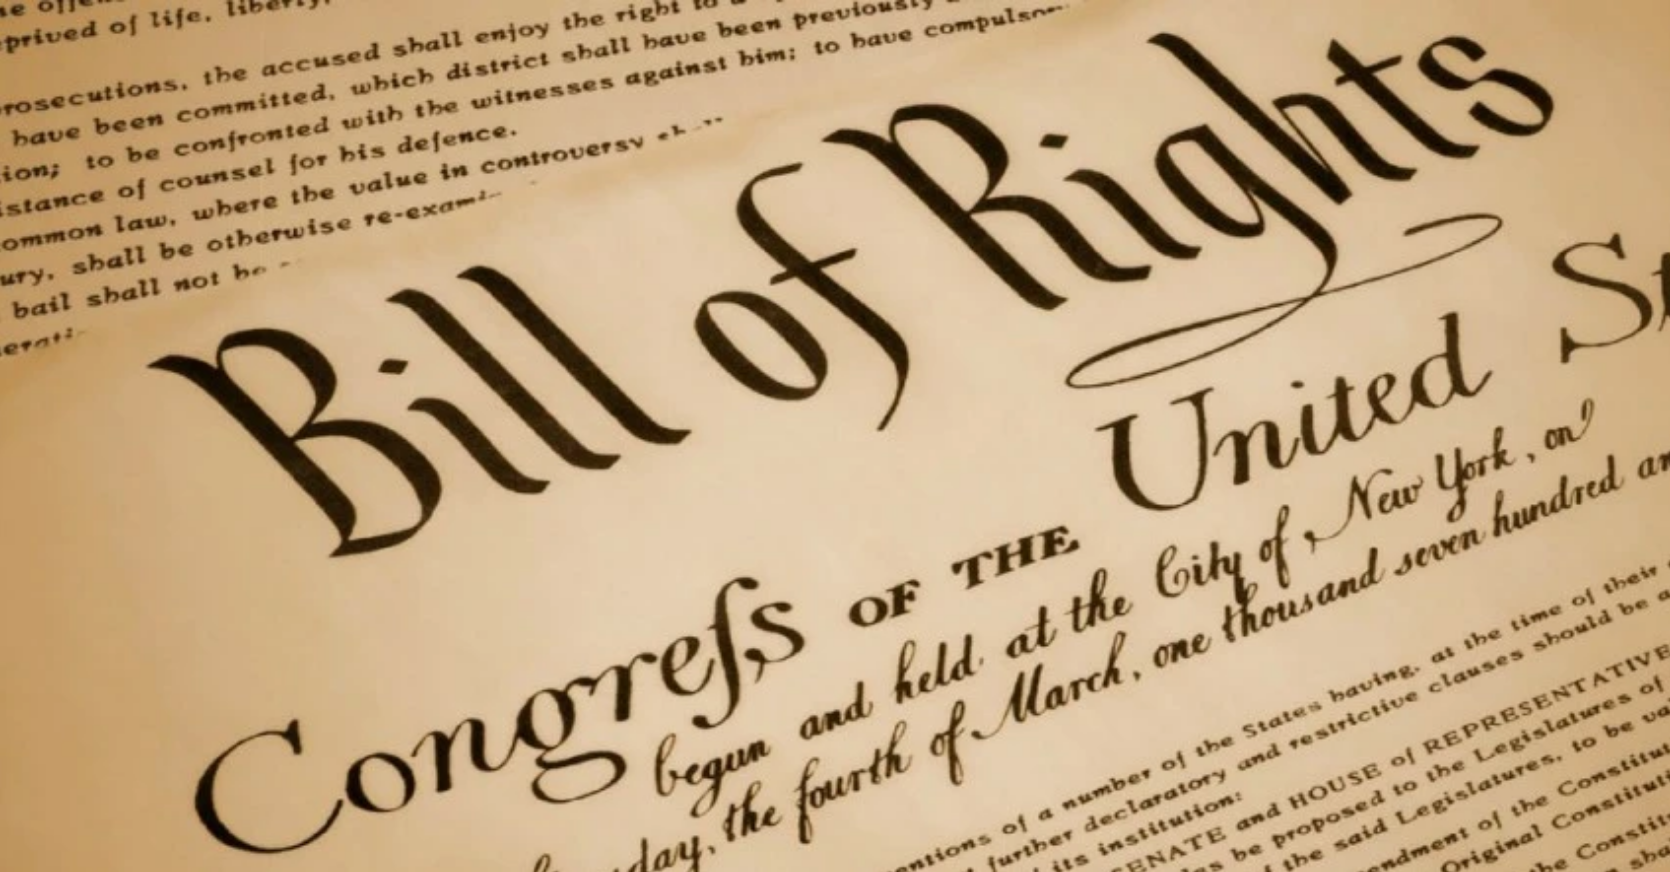
\includegraphics[width=1.0\paperwidth]{bill_of_rights.png}}
  \begin{frame}[plain]
  
%\begin{mdframed}[tikzsetting={draw=black,fill=white,fill opacity=0.7,
%               line width=0pt},backgroundcolor=none,leftmargin=0,
%               rightmargin=40,innertopmargin=4pt]
%\Huge Optimal Turbine Inspections
%\end{mdframed}

  \end{frame}
}

%@@@@@@@@@@@@@@@@@@@@@@@@@@@@@@@@@@@@@@@@@@@@@@@@@
\begin{frame}

\begin{center}
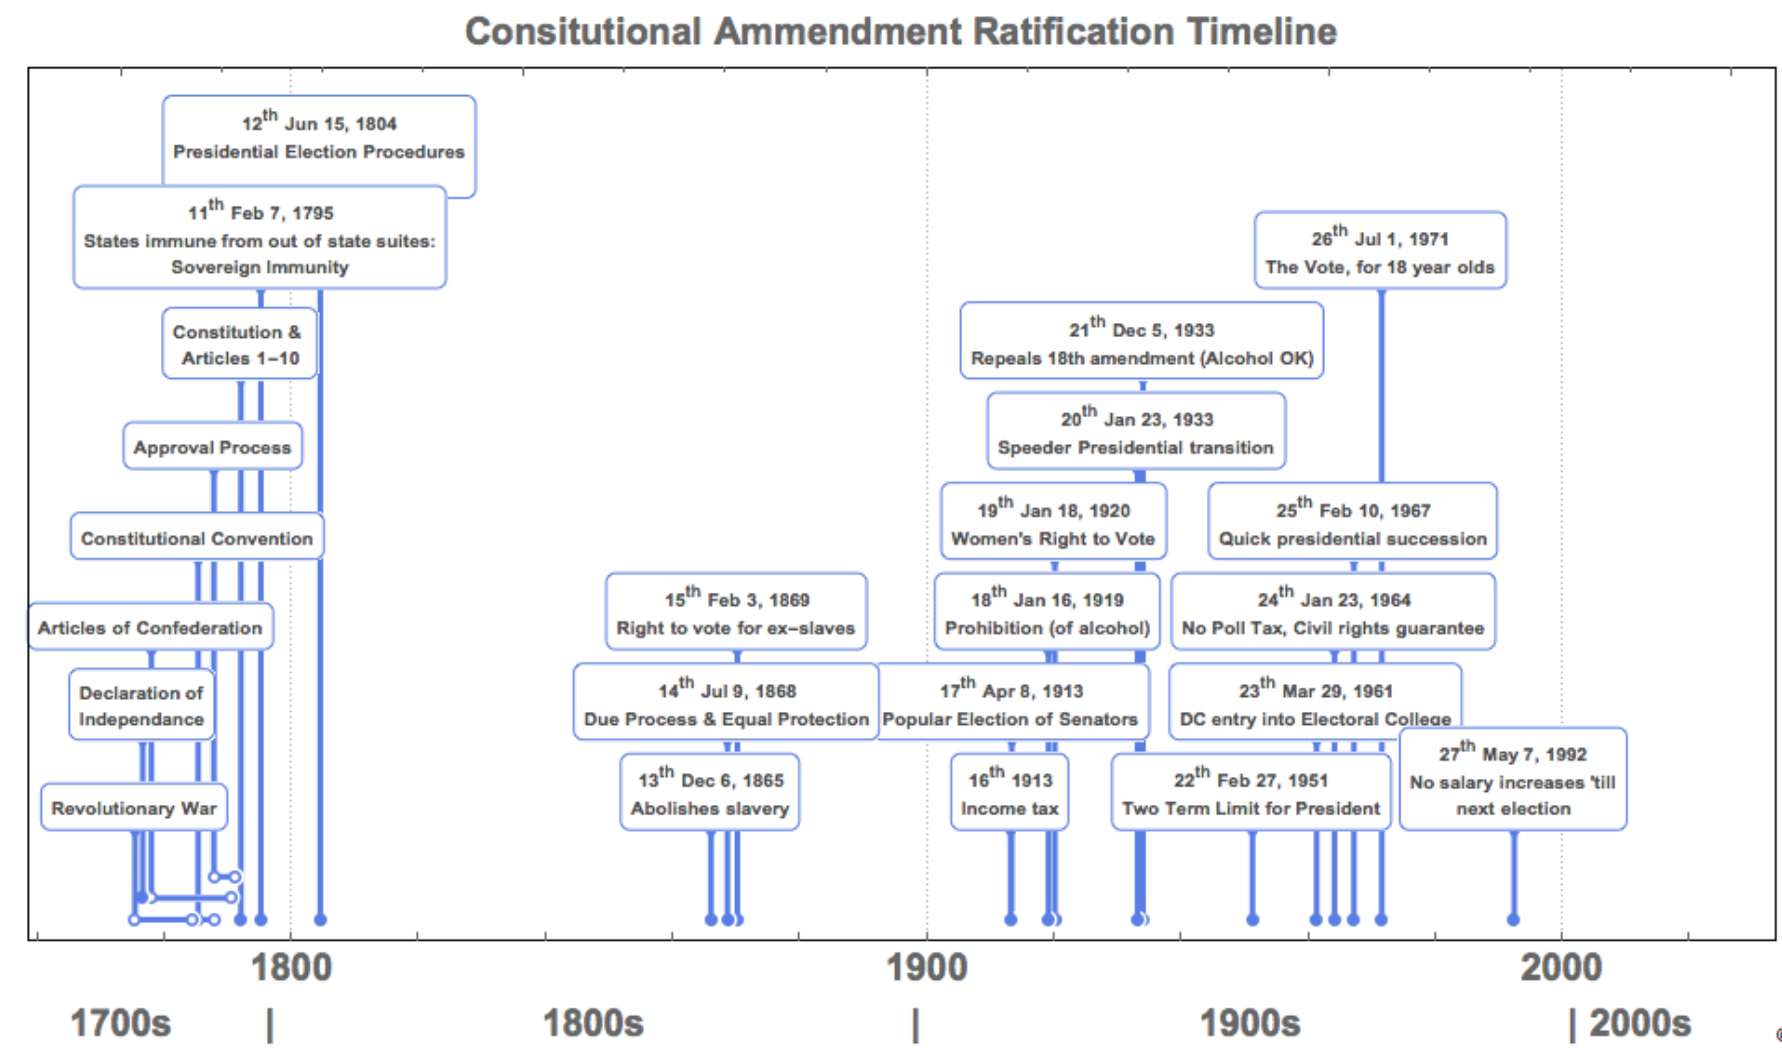
\includegraphics[scale=0.4]{Amendment_timeline.png}
\end{center}


\end{frame}

%@@@@@@@@@@@@@@@@@@@@@@@@@@@@@@@@@@@@@@@@@@@@@@@@@
\begin{frame}
\frametitle{Bill of Rights}

\begin{itemize}
\item Individual rights (Amendments 1-8);
\bigskip
\bigskip
\item Unenumerated powers (9);
\bigskip
\bigskip
\item Reserved powers (10);
\bigskip
\bigskip
\item Madison's baby, inspired by the Magna Carta (1215), the English Bill of Rights (1689), and state constitutions; a compromise between the federalists and the anti-federalists;
\end{itemize}

\end{frame}

%@@@@@@@@@@@@@@@@@@@@@@@@@@@@@@@@@@@@@@@@@@@@@@@@@
\begin{frame}
\frametitle{Bill of Rights: 1st Amendment (1791, free speech)}

Congress shall make no law respecting an establishment of religion, or prohibiting the free exercise thereof; or abridging the freedom of speech, or of the press; or the right of the people peaceably to assemble, and to petition the government for a redress of grievances.
\bigskip
\begin{itemize}
\item Initially interpreted more narrowly than it is today;
\item Applied in Near v. Minnesota (1931), Everson v. Board of Education (1947), New York Times Co. v. Sullivan (1964), New York Times v. United States (1971).
\end{itemize}
\end{frame}

%@@@@@@@@@@@@@@@@@@@@@@@@@@@@@@@@@@@@@@@@@@@@@@@@@
\begin{frame}
\frametitle{Bill of Rights: 2nd Amendment (1791, right to bear arms)}
A well regulated militia, being necessary to the security of a free state, the right of the people to keep and bear arms, shall not be infringed.\\
\bigskip
In the 2008 case District of Columbia v. Heller, the Supreme Court held that ``the Second Amendment protects an individual right to possess a firearm unconnected with service in a militia, and to use that arm for traditionally lawful purposes, such as self-defense within the home."
\bigskip
\begin{itemize}
\item Controversial - basis in the English Bill of Rights (1689);
\item United States v. Cruikshank (1876), United States v. Miller (1939), District of Columbia v. Heller (2008), McDonald v. Chicago (2010).
\end{itemize}

\end{frame}

%@@@@@@@@@@@@@@@@@@@@@@@@@@@@@@@@@@@@@@@@@@@@@@@@@
\begin{frame}
\frametitle{Bill of Rights: 3rd Amendment (1791, no quartering soldiers)}
No Soldier shall, in time of peace be quartered in any house, without the consent of the Owner, nor in time of war, but in a manner to be prescribed by law.
\bigskip
\begin{itemize}
\item Informed by experience during the revolution - uncontroversial today;
\item Has never been the primary basis for a supreme court decision.
\end{itemize}

\end{frame}

%@@@@@@@@@@@@@@@@@@@@@@@@@@@@@@@@@@@@@@@@@@@@@@@@@
\begin{frame}
\frametitle{Bill of Rights: 4th Amendment (1791, no unreasonable search and seizure)}
The right of the people to be secure in their persons, houses, papers, and effects, against unreasonable searches and seizures, shall not be violated, and no Warrants shall issue, but upon probable cause, supported by Oath or affirmation, and particularly describing the place to be searched, and the persons or things to be seized.
\bigskip
\begin{itemize}
\item Also informed by colonial experience - response to the abuse of the writ of assistance;
\item Cited in numerous Supreme Court decisions.
\end{itemize}

\end{frame}

%@@@@@@@@@@@@@@@@@@@@@@@@@@@@@@@@@@@@@@@@@@@@@@@@@
\begin{frame}
\frametitle{Bill of Rights: 5th Amendment (1791, rights of persons)}
No person shall be held to answer for a capital, or otherwise infamous crime, unless on a presentment or indictment of a Grand Jury, except in cases arising in the land or naval forces, or in the Militia, when in actual service in time of War or public danger; nor shall any person be subject for the same offense to be twice put in jeopardy of life or limb; nor shall be compelled in any criminal case to be a witness against himself, nor be deprived of life, liberty, or property, without due process of law; nor shall private property be taken for public use, without just compensation.
\bigskip
\begin{itemize}
\item Basis for Miranda rights, i.e. `You have the right to remain silent...' established in Miranda v. Arizona (1966).
\end{itemize}

\end{frame}

%@@@@@@@@@@@@@@@@@@@@@@@@@@@@@@@@@@@@@@@@@@@@@@@@@
\begin{frame}
\frametitle{Bill of Rights: 6th Amendment (1791, rights of the accused)}
In all criminal prosecutions, the accused shall enjoy the right to a speedy and public trial, by an impartial jury of the State and district wherein the crime shall have been committed, which district shall have been previously ascertained by law, and to be informed of the nature and cause of the accusation; to be confronted with the witnesses against him; to have compulsory process for obtaining witnesses in his favor, and to have the Assistance of Counsel for his defence.
\bigskip
\begin{itemize}
\item Used to argue for right to legal representation, established in Gideon v. Wainwright (1963).
\end{itemize}

\end{frame}

%@@@@@@@@@@@@@@@@@@@@@@@@@@@@@@@@@@@@@@@@@@@@@@@@@
\begin{frame}
\frametitle{Bill of Rights: 7th Amendment (1791, civil trials)}
In Suits at common law, where the value in controversy shall exceed twenty dollars, the right of trial by jury shall be preserved, and no fact tried by a jury, shall be otherwise re-examined in any Court of the United States, than according to the rules of the common law.
\bigskip
\begin{itemize}
\item An olive branch to Anti-Federalists;
\item Practical effect was to deny the Supreme Court the power to overrule jury trials regarding findings of fact.
\end{itemize}

\end{frame}

%@@@@@@@@@@@@@@@@@@@@@@@@@@@@@@@@@@@@@@@@@@@@@@@@@
\begin{frame}
\frametitle{Bill of Rights: 8th Amendment (1791, no cruel or unusual punishments)}
Excessive bail shall not be required, nor excessive fines imposed, nor cruel and unusual punishments inflicted.
\bigskip
\begin{itemize}
\item Inspired by case of Titus Oates (and maybe stuff like Hanging, Drawing, and Quartering);
\item `cruel and unusual' the most frequently litigated clause;
\item Some Supreme Court Justices argued that capital punishment itself failed this test in Furman v. Georgia (1972).
\end{itemize}

\end{frame}

%@@@@@@@@@@@@@@@@@@@@@@@@@@@@@@@@@@@@@@@@@@@@@@@@@
\begin{frame}
\frametitle{Bill of Rights: 9th Amendment (1791, unlisted rights)}
The enumeration in the Constitution, of certain rights, shall not be construed to deny or disparage others retained by the people.
\bigskip
\begin{itemize}
\item Declaration that additional fundamental rights exist outside the constitution;
\item Basis of Roe v. Wade (1973).
\end{itemize}

\end{frame}

%@@@@@@@@@@@@@@@@@@@@@@@@@@@@@@@@@@@@@@@@@@@@@@@@@
\begin{frame}
\frametitle{Bill of Rights: 10th Amendment (1791, reserved powers)}
The powers not delegated to the United States by the Constitution, nor prohibited by it to the States, are reserved to the States respectively, or to the people.
\bigskip
\begin{itemize}
\item A denial of implied powers and a reinforcement of Federalism;
\item Has been characterized as a truism.
\end{itemize}

\end{frame}

%@@@@@@@@@@@@@@@@@@@@@@@@@@@@@@@@@@@@@@@@@@@@@@@@@
\begin{frame}
\frametitle{11th Amendment (1795, suits against the states)}
The Judicial power of the United States shall not be construed to extend to any suit in law or equity, commenced or prosecuted against one of the United States by Citizens of another State, or by Citizens or Subjects of any Foreign State.

\end{frame}

%@@@@@@@@@@@@@@@@@@@@@@@@@@@@@@@@@@@@@@@@@@@@@@@@@
\begin{frame}
\frametitle{12th Amendment (1804, POTUS and VP run together)}
...President and vice president run together...
\end{frame}

%@@@@@@@@@@@@@@@@@@@@@@@@@@@@@@@@@@@@@@@@@@@@@@@@@
\begin{frame}
\frametitle{13th Amendment (1865, slavery only in prisons)}
Neither slavery nor involuntary servitude, except as a punishment for crime whereof the party shall have been duly convicted, shall exist within the United States, or any place subject to their jurisdiction.
\end{frame}

%@@@@@@@@@@@@@@@@@@@@@@@@@@@@@@@@@@@@@@@@@@@@@@@@@
\begin{frame}
\frametitle{14th Amendment (1868, due process and equal protection)}
All persons born or naturalized in the United States, and subject to the jurisdiction thereof, are citizens of the United States and of the state wherein they reside. No state shall make or enforce any law which shall abridge the privileges or immunities of citizens of the United States; nor shall any state deprive any person of life, liberty, or property, without due process of law; nor deny to any person within its jurisdiction the equal protection of the laws.\\
\bigskip
Representatives shall be apportioned among the several states according to their respective numbers, counting the whole number of persons in each state, excluding Indians not taxed.
\end{frame}

%@@@@@@@@@@@@@@@@@@@@@@@@@@@@@@@@@@@@@@@@@@@@@@@@@
\begin{frame}
\frametitle{15th Amendment (1870, citizens' voting rights)}
The right of citizens of the United States to vote shall not be denied or abridged by the United States or by any state on account of race, color, or previous condition of servitude.
\end{frame}

%@@@@@@@@@@@@@@@@@@@@@@@@@@@@@@@@@@@@@@@@@@@@@@@@@
\begin{frame}
\frametitle{16th Amendment (1913, federal income tax)}
The Congress shall have power to lay and collect taxes on incomes, from whatever source derived, without apportionment among the several States, and without regard to any census or enumeration.
\end{frame}

%@@@@@@@@@@@@@@@@@@@@@@@@@@@@@@@@@@@@@@@@@@@@@@@@@
\begin{frame}
\frametitle{17th Amendment (1913, popular election of senators)}
The Senate of the United States shall be composed of two Senators from each State, elected by the people thereof, for six years; and each Senator shall have one vote. The electors in each State shall have the qualifications requisite for electors of the most numerous branch of the State legislatures.
\end{frame}

%@@@@@@@@@@@@@@@@@@@@@@@@@@@@@@@@@@@@@@@@@@@@@@@@@
\begin{frame}
\frametitle{18th Amendment (1919, prohibition)}
After one year from the ratification of this article the manufacture, sale, or transportation of intoxicating liquors within, the importation thereof into, or the exportation thereof from the United States and all the territory subject to the jurisdiction thereof for beverage purposes is hereby prohibited. 
\end{frame}

%@@@@@@@@@@@@@@@@@@@@@@@@@@@@@@@@@@@@@@@@@@@@@@@@@
\begin{frame}
\frametitle{19th Amendment (1920, womens' suffrage)}
The right of citizens of the United States to vote shall not be denied or abridged by the United States or by any State on account of sex.
\begin{itemize}
\item Husted and Kenny (1997) find it led to a rise in welfare spending.
\item Miller (2008) shows that child mortality was reduced since women's suffrage resulted in increasing state-level spending on programs related to the health of infants and children.
\item Zhang (2019) finds that it decreased polarization.
\end{itemize}
\end{frame}

%@@@@@@@@@@@@@@@@@@@@@@@@@@@@@@@@@@@@@@@@@@@@@@@@@
\begin{frame}
\frametitle{20th Amendment (1933, less lame duck)}
The terms of the President and Vice President shall end at noon on the 20th day of January, and the terms of Senators and Representatives at noon on the 3d day of January, of the years in which such terms would have ended if this article had not been ratified; and the terms of their successors shall then begin. 
\end{frame}

%@@@@@@@@@@@@@@@@@@@@@@@@@@@@@@@@@@@@@@@@@@@@@@@@@
\begin{frame}
\frametitle{21st Amendment (1933, no prohibition!)}
The eighteenth article of amendment to the Constitution of the United States is hereby repealed. 
\end{frame}

%@@@@@@@@@@@@@@@@@@@@@@@@@@@@@@@@@@@@@@@@@@@@@@@@@
\begin{frame}
\frametitle{22nd Amendment (1951, presidential term limits)}
No person shall be elected to the office of the President more than twice, and no person who has held the office of President, or acted as President, for more than two years of a term to which some other person was elected President shall be elected to the office of the President more than once.
\end{frame}

%@@@@@@@@@@@@@@@@@@@@@@@@@@@@@@@@@@@@@@@@@@@@@@@@@
\begin{frame}
\frametitle{23rd Amendment (1961, DC electors)}
The District constituting the seat of Government of the United States shall appoint in such manner as the Congress may direct: A number of electors of President and Vice President equal to the whole number of Senators and Representatives in Congress to which the District would be entitled if it were a State...
\end{frame}

%@@@@@@@@@@@@@@@@@@@@@@@@@@@@@@@@@@@@@@@@@@@@@@@@@
\begin{frame}
\frametitle{24th Amendment (1964, no more poll tax)}
The right of citizens of the United States to vote in any primary or other election for President or Vice President, for electors for President or Vice President, or for Senator or Representative in Congress, shall not be denied or abridged by the United States or any State by reason of failure to pay any poll tax or other tax.
\begin{center}
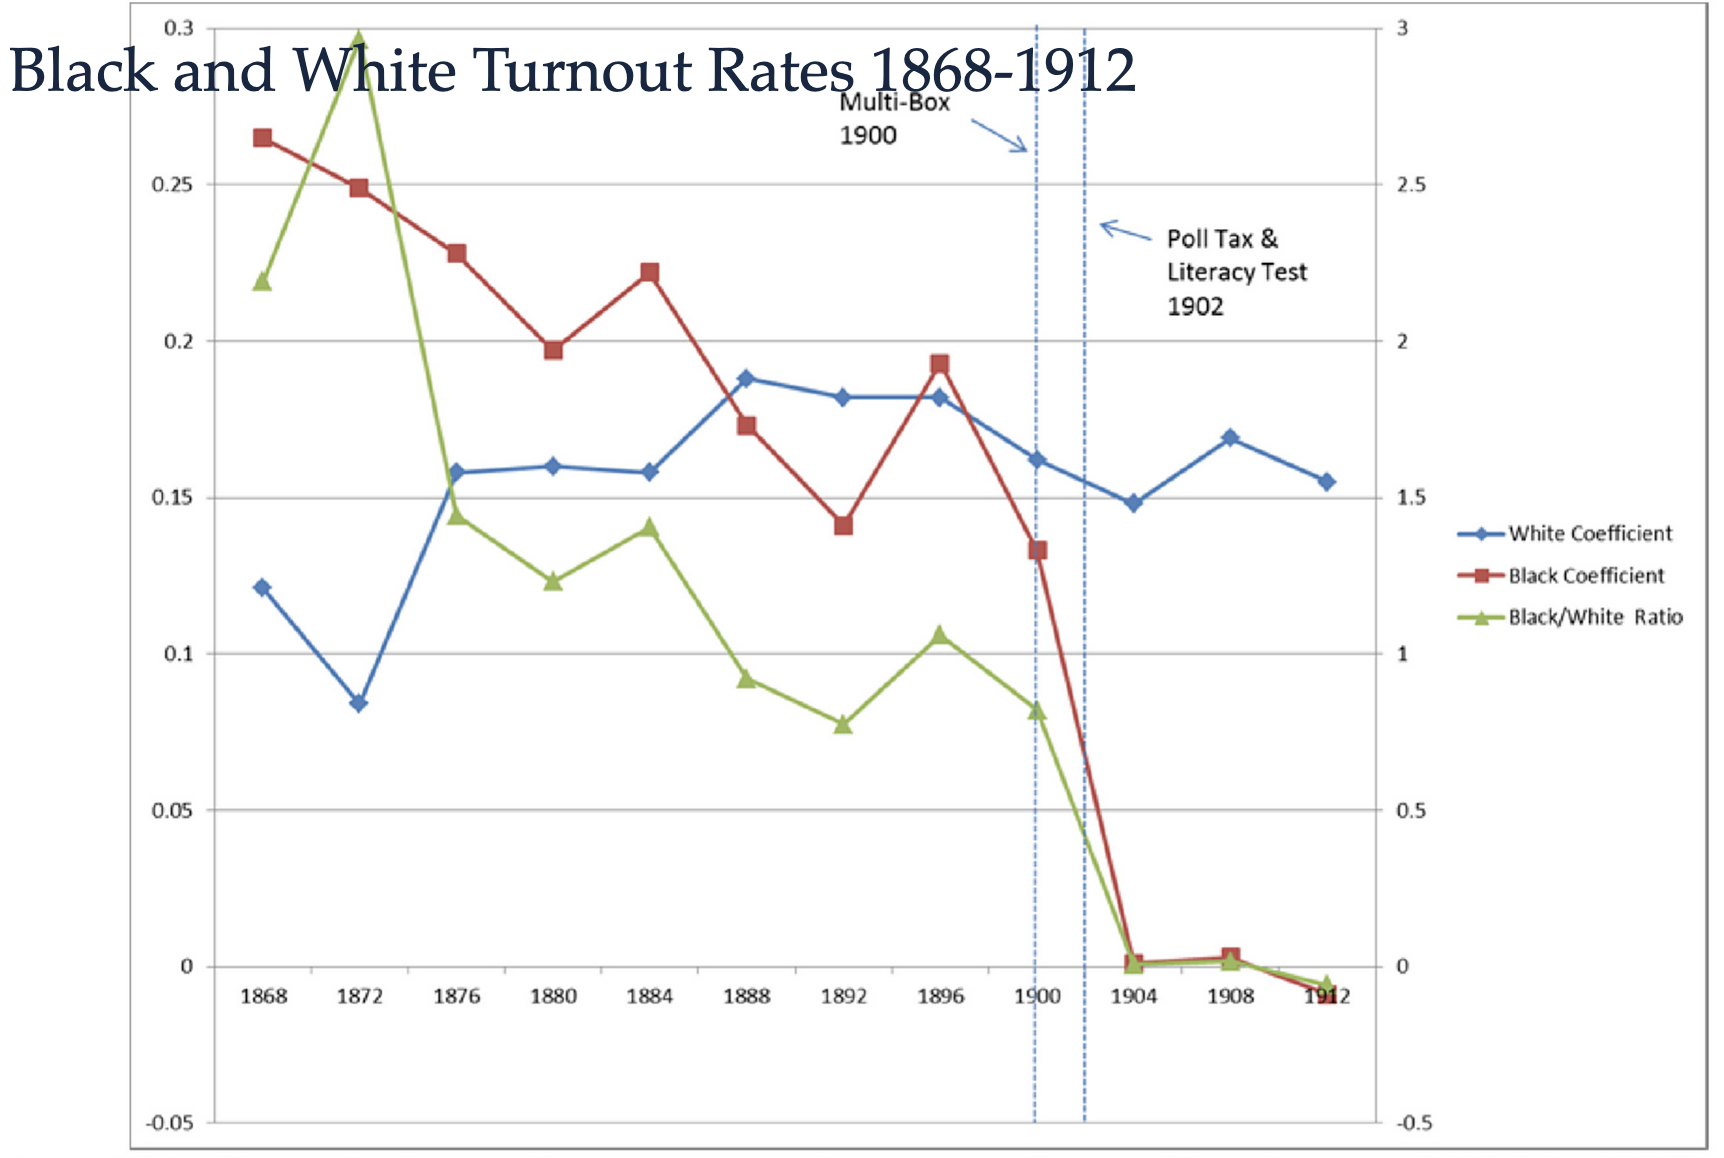
\includegraphics[scale=0.25]{black_white_turnout.png}
\end{center}

\end{frame}

%@@@@@@@@@@@@@@@@@@@@@@@@@@@@@@@@@@@@@@@@@@@@@@@@@
\begin{frame}
\frametitle{25th Amendment (1967, presidential succession)}
In case of the removal of the President from office or of his death or resignation, the Vice President shall become President.
\begin{center}
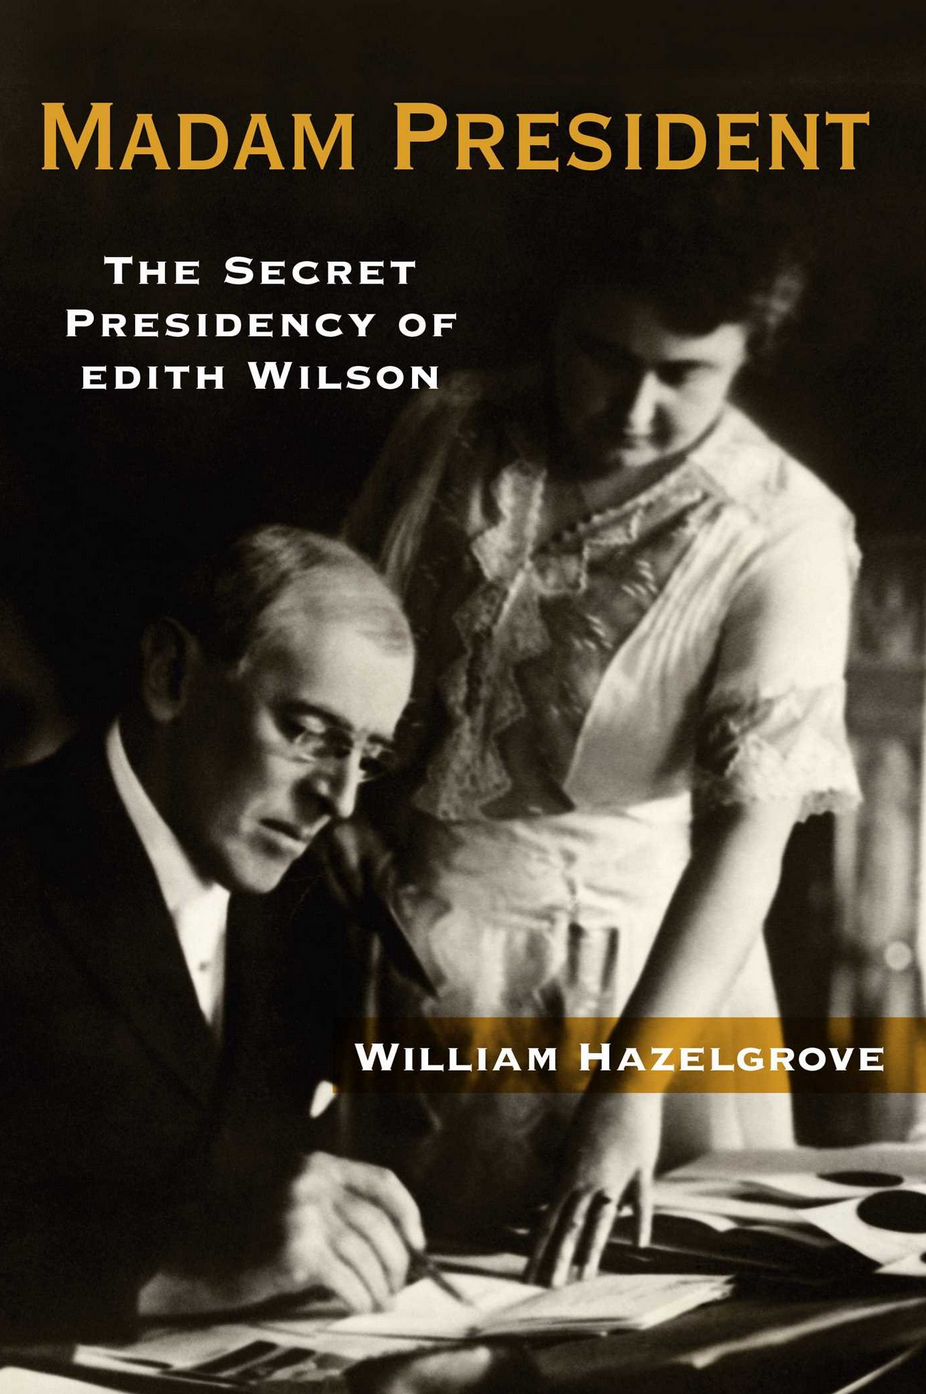
\includegraphics[scale=0.25]{madam_president.png}
\end{center}

\end{frame}

%@@@@@@@@@@@@@@@@@@@@@@@@@@@@@@@@@@@@@@@@@@@@@@@@@
\begin{frame}
\frametitle{26th Amendment (1971, voting age)}
The right of citizens of the United States, who are eighteen years of age or older, to vote shall not be denied or abridged by the United States or by any State on account of age. 
\end{frame}

%@@@@@@@@@@@@@@@@@@@@@@@@@@@@@@@@@@@@@@@@@@@@@@@@@
\begin{frame}
\frametitle{27th Amendment (1992, congress can't raise its own pay)}
No law varying the compensation for the services of the Senators and Representatives shall take effect, until an election of Representatives shall have intervened.
\end{frame}

%@@@@@@@@@@@@@@@@@@@@@@@@@@@@@@@@@@@@@@@@@@@@@@@@@
\begin{frame}
\frametitle{Unratified Amendments}
\begin{itemize}
\item Congressional Apportionment Amendment (1789)
\bigskip
\item Titles of Nobility Amendment (1810)
\bigskip
\item Corwin Amendment (1861)
\bigskip
\item Child Labor Amendment (1924)
\bigskip
\item Equal Rights Amendment (1923)
\bigskip
\item District of Columbia Voting Rights Amendment (1978)
\end{itemize}
\end{frame}


%@@@@@@@@@@@@@@@@@@@@@@@@@@@@@@@@@@@@@@@@@@@@@@@@@
\begin{frame}
\frametitle{Final thoughts}

\begin{itemize}
\item Above all: the US constitution is a policy for making policies.
\bigskip
\item How `live' should the constitution be?
\bigskip
\item What rises to the level of an amendment?\onslide<2->
\bigskip
\begin{enumerate}
\item change to HOW we make policy;
\bigskip
\item laws that would be unconstitutional given the current structure;
\end{enumerate}
\bigskip
\item Why do we fail to make amendments?  Because the people want them and congress fails to propose them (not ok) or because congress correctly assesses the people do not want them (prob ok)?
\bigskip
\item What is in your constitutional objective function?
\end{itemize}

\end{frame}


\end{document}








